%!TEX root = ../template.tex
%%%%%%%%%%%%%%%%%%%%%%%%%%%%%%%%%%%%%%%%%%%%%%%%%%%%%%%%%%%%%%%%%%%%
%% chapter3.tex
%% NOVA thesis document file
%%
%% Chapter with a short latex tutorial and examples
%%%%%%%%%%%%%%%%%%%%%%%%%%%%%%%%%%%%%%%%%%%%%%%%%%%%%%%%%%%%%%%%%%%%

\typeout{NT FILE chapter3.tex}%

\chapter{State Of The Art}
\label{cha:State_Of_The_Art}

\section{Certified Compilers}
\label{sec:Certified_Compilers}

\subsection{CompCert}
\label{sec:CompCert}

\subsection{CakeML}
\label{sec:CakeML}

%% https://github.com/CakeML/cakeml/blob/master/how-to.md

%%lets terminam com end e nao esta a acontecer na extracao
%%literais boleanos comecam com letra grande
%%cakeml nao suportam loops sem ser recursivos
%%Ref e com letra grande
%%datatypes ficam todos mal feitos e trocados
%%operacoes com arrays nao funciona bem na traducao
%%expections sao definidas fora da funcao

\section{Pipeline}
\label{sec:Pipeline}

Some parts of the verification pipeline have already been implemented or require only minor adjustments to meet their 
objectives. As we know, Cameleer provides translation of OCaml code annotated with GOSPEL specifications into WhyML. 
This extraction process succeeds when the OCaml code and its accompanying specifications are correctly written. However, 
it is not designed to prevent users from extracting code even if the GOSPEL specifications are incomplete or insufficient 
to guarantee correctness. Below is a draft overview of the pipeline.

\begin{figure}[H]
    \centering
    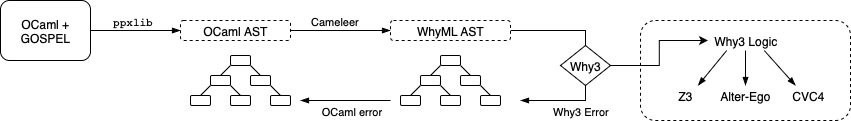
\includegraphics[width=\linewidth]{images/Cameleer_OCaml_WhyML.png}
    \caption{OCaml to WhyML pipeline with cameleer}

\end{figure}

By modifying the extraction process in Cameleer, we could potentially generate CakeML code directly from OCaml. 
However, the current extraction is not designed for this purpose and would produce incorrect CakeML code. This is not 
only due to differences in syntax but also because some OCaml features have no direct equivalents in CakeML, making a 
straightforward translation impossible without further adaptation.

\begin{figure}[H]
    \centering
    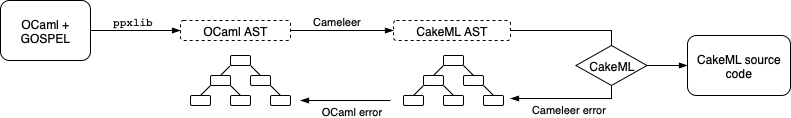
\includegraphics[width=\linewidth]{images/Cameleer_OCaml_CakeML.png}
    \caption{OCaml to CakeML pipeline with cameleer change}

\end{figure}

The goal pipeline for this paper is to translate code from OCaml and GOSPEL specifications into WhyML, where it can 
be verified using the various automated provers available in Why3. Once the code is proven correct in WhyML, it can 
then be translated into CakeML, applying the necessary syntax adjustments and providing error feedback for any constructs 
that cannot be translated.

\begin{figure}[H]
    \centering
    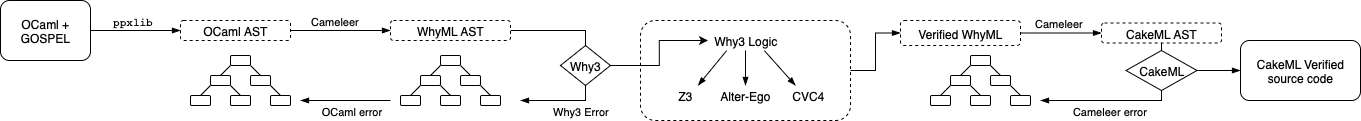
\includegraphics[width=\linewidth]{images/Cameleer_OCaml_WhyML_CakeML.png}
    \caption{Goal pipeline}

\end{figure}

\begin{figure}[H]
    \centering
    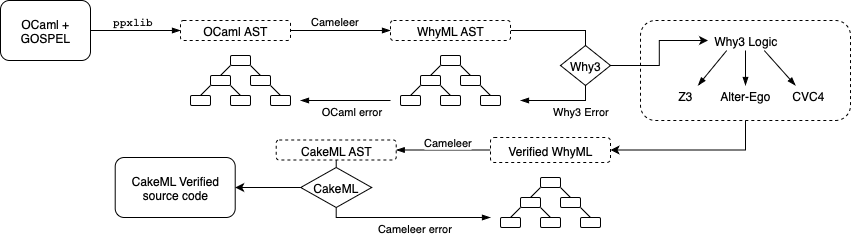
\includegraphics[width=\linewidth]{images/Goal_Pipeline.png}
    \caption{Goal pipeline}

\end{figure}

%%existe extracao cameleer para whyml, de whyml para cakeml, whyml para ocaml64